\documentclass[12pt]{article}
\usepackage[margin=1in]{geometry}
\usepackage{amsmath, amssymb}
\usepackage{graphicx}
\usepackage{booktabs}
\usepackage{caption}
\usepackage[colorlinks=true, linkcolor=blue, citecolor=blue, urlcolor=blue]{hyperref}
\usepackage{setspace}
\usepackage[numbers,sort&compress]{natbib}
\usepackage{microtype}
\usepackage{times}
\usepackage{array}
\usepackage{float}
\graphicspath{{figures/}}

\setlength{\parindent}{0pt}
\setlength{\parskip}{8pt}
\onehalfspacing

\begin{document}

% ===========================================================================
% TITLE PAGE
% ===========================================================================
\begin{titlepage}
\centering
\vspace*{1cm}

{\large\bfseries Scaling Laws and Conditional Generation in Diffusion Protein\\[6pt]
Language Models for T-Cell Receptor Design}

\vspace{1.5cm}


\includegraphics[width=0.4\textwidth]{ASU-logo.png}\\[1cm]

{\large Anuj Prabhu}

\vspace{0.5cm}

{\normalsize School of Computing and Augmented Intelligence}

{\normalsize Barrett, The Honors College}

{\normalsize Arizona State University}

\vspace{1cm}

{\normalsize\itshape Faculty Director}

{\normalsize Dr.\ Heewook Lee}

\vspace{0.5cm}

{\normalsize\itshape Second Committee Member}

{\normalsize Pengfei Zhang}

\vspace{1.5cm}

{\normalsize\itshape Barrett Undergraduate Honors Thesis}

{\normalsize Spring 2026}

\end{titlepage}

% ===========================================================================
% ABSTRACT
% ===========================================================================
\newpage
\section*{Abstract}

T-cell receptors (TCRs) mediate antigen recognition in adaptive immunity, and the ability to
computationally generate TCRs with defined epitope specificity would accelerate vaccine design
and cancer immunotherapy. The complementarity-determining region 3 (CDR3) of the TCR beta
chain is the primary determinant of antigen specificity and the key target for engineering
TCR-epitope recognition, yet its sequence space spans an estimated $10^{15}$ unique
sequences, making comprehensive experimental exploration intractable.
Generative models offer a path forward, yet the scaling behavior of protein diffusion
models (how performance improves with model capacity and training data) remains largely
uncharacterized.

We train models using the DPLM framework~\cite{wang2024dplm} across five model
sizes (0.1M--50M parameters) and four dataset sizes (500K--32M TCR sequences),
characterizing how validation loss follows the power law $L(N) = a \cdot N^{-\alpha} + c$.
Pretraining exponents $\alpha$ range from 0.39 to 0.77 across dataset sizes. We further
develop a supervised fine-tuning (SFT) procedure for epitope-conditioned TCR generation and
find that SFT scaling exponents ($\alpha = 0.68$--$0.74$) consistently exceed pretraining
exponents, indicating that model scale is a more effective lever for conditional generation than for
unconditional pretraining. Generation quality measured via TCR-BERT~\cite{wu2021tcrbert} pseudo-log-likelihood
improves monotonically with model scale.

\begin{center}
\textbf{Repository:} \url{https://github.com/anujprabhu01/honors-thesis-dplm-tcr-scaling}
\end{center}

% ===========================================================================
% TABLE OF CONTENTS
% ===========================================================================
\newpage
\tableofcontents

% ===========================================================================
% INTRODUCTION
% ===========================================================================
\newpage
\section{Introduction}

The adaptive immune system relies on T-lymphocytes to detect and destroy
pathogen-infected and malignant cells. Central to this process is the T-cell receptor (TCR),
a surface-expressed heterodimer that surveys peptides presented on major histocompatibility
complex (MHC) molecules. The complementarity-determining region 3 (CDR3) of the TCR beta
chain is the primary contact interface with the peptide-MHC complex and therefore the dominant
determinant of antigen specificity~\cite{davis1988}. Harnessing this specificity
computationally (identifying or designing TCRs that recognize a given target epitope) has
broad applications in cancer immunotherapy, infectious disease vaccine design, and the study
of autoimmunity~\cite{june2018}.

A fundamental challenge is the extraordinary diversity of the TCR sequence space. Combinatorial
VDJ recombination and junctional diversity generate an estimated $10^{15}$ unique CDR3 beta
chain sequences per individual, of which only a small fraction can be assayed
experimentally~\cite{robins2009}. High-throughput immune repertoire sequencing has enabled the
collection of large TCR databases, creating an opportunity for data-driven generative modeling.
If a generative model can learn the statistical structure of TCR sequences and then be directed
toward a specific target epitope, it could substantially accelerate the identification of
candidate sequences for therapeutic or research applications.

Protein language models have emerged as powerful tools for sequence-level modeling. Autoregressive
models such as ProtGPT2~\cite{ferruz2022} have been applied to protein generation with promising
results. Masked language models such as ESM-2~\cite{lin2023} have demonstrated strong
representation learning capabilities. The DPLM model~\cite{wang2024dplm} extends the absorbing discrete diffusion
framework~\cite{austin2021} to protein sequences, iteratively denoising randomly masked tokens
using a transformer backbone, and has shown strong generative and predictive performance.

Despite these advances, two critical gaps remain. First, the scaling behavior of protein
diffusion models (the systematic relationship between model size, dataset size, and generation
quality) has not been characterized. In natural language processing, power law scaling
relationships are well-established: validation loss decreases predictably as a power law in
both model parameters and training tokens~\cite{kaplan2020, hoffmann2022}. Whether similar
laws hold for discrete protein diffusion models trained on domain-specific sequence data is
an open question with practical implications for resource allocation and model design. Second,
most existing TCR generative models operate unconditionally or rely on retrieval-based methods,
rather than learning to generate TCR sequences conditioned on a specific target epitope.

This thesis addresses both gaps. We conduct a systematic scaling study of DPLM models trained on
TCR CDR3 beta chain sequences, varying model size from 0.1M to 50M parameters across four
dataset sizes (500K, 2M, 8M, and 32M sequences). We fit power law scaling curves to
characterize how validation loss scales with model size at each dataset size, and we develop
a supervised fine-tuning (SFT) procedure for epitope-conditioned generation. Generated TCRs
are evaluated using three complementary approaches: binding affinity prediction (BAP),
sequence-level similarity to known binders (TCRMatch~\cite{chronister2021}), and
TCR-BERT~\cite{wu2021tcrbert} pseudo-log-likelihood (PLL).

\subsection{Background}

\textbf{TCR structure and CDR3 biology.}
The TCR is a disulfide-linked heterodimer composed of alpha and beta chains, each encoded by
variable (V), diversity (D), and joining (J) gene segments joined by junctional nucleotides
to produce CDR3 loops of variable length and sequence. The CDR3 beta chain (CDR3$\beta$),
typically 10--20 amino acids in length with a conserved CASS prefix, is the primary
determinant of peptide-MHC recognition specificity~\cite{davis1988}. This work models the
CDR3$\beta$ sequence as a proxy for TCR identity and specificity.

\textbf{Protein language models.}
Large-scale masked language models (MLMs) trained on protein sequence databases have emerged
as powerful encoders and generators~\cite{lin2023, devlin2019}. ESM-2~\cite{lin2023} trains a
transformer with the BERT-style masked language modeling objective on hundreds of millions of
UniRef sequences, yielding representations that correlate with protein structure and function.
We adopt the ESM-2 transformer architecture as the backbone for our DPLM models, training from
scratch on TCR sequences rather than loading pretrained weights.

\textbf{Absorbing discrete diffusion.}
Discrete diffusion models operate in token space rather than a continuous latent space. Following
Austin et al.~\cite{austin2021}, the forward process gradually replaces tokens with a special
MASK token at a rate proportional to a sampled diffusion timestep $t \sim \text{Uniform}[1, T]$.
The model is trained to recover the original tokens from the partially masked sequence, using a
cross-entropy loss over masked positions. At inference, a sequence of all MASK tokens is
iteratively refined over $T$ steps. DPLM~\cite{wang2024dplm} instantiates this framework using
the ESM-2 transformer, demonstrating competitive performance on protein generation and
representation learning tasks.

\textbf{Neural scaling laws.}
Kaplan et al.~\cite{kaplan2020} established that validation loss in autoregressive language
models follows a power law in model parameters $N$ and training tokens $D$:
$L(N) = a \cdot N^{-\alpha}$ and $L(D) = b \cdot D^{-\beta}$, with observed exponents
$\alpha \approx 0.076$ and $\beta \approx 0.095$ for GPT-scale models trained on English text.
Hoffmann et al.~\cite{hoffmann2022} (Chinchilla) subsequently showed that compute-optimal
training requires approximately $D \approx 20N$ training tokens per model parameter, revising
earlier scaling predictions. Whether analogous scaling laws hold for protein diffusion models
on domain-specific sequence data is unknown and is a central question of this thesis.

\textbf{TCR evaluation methods.}
TCRMatch~\cite{chronister2021} evaluates generated TCRs by computing BLOSUM62-weighted k-mer
similarity to real TCRs known to bind each epitope, quantifying sequence-level similarity to
known binders. Binding affinity prediction (BAP) models, including retrained versions of
NetTCR~\cite{montemurro2022} (CNN) and ERGO~\cite{springer2020} (LSTM), estimate the
probability that a generated TCR binds its target epitope. TCR-BERT~\cite{wu2021tcrbert} is a
masked language model pretrained on TCR sequences; its pseudo-log-likelihood (PLL), computed
by individually masking each position, provides a model-based estimate of sequence plausibility.

% ===========================================================================
% METHODS
% ===========================================================================
\section{Methods}

\subsection{Model Architecture}

We trained DPLM models using the ESM-2 transformer architecture~\cite{lin2023} with five
configurations spanning 0.1M to 50M parameters, as summarized in Table~\ref{tab:arch}. All
models used sinusoidal positional embeddings with maximum sequence length 1,026, a vocabulary
of 33 tokens (20 standard amino acids plus special tokens), and dropout of 0.1. Model weights
were initialized randomly (no pretrained ESM-2 weights were loaded), consistent with training
models from scratch on TCR sequence data. The number of diffusion timesteps was set to $T = 500$
for all configurations.

\begin{table}[H]
\centering
\caption{DPLM model architecture configurations. Hidden: hidden dimension size. Layers: number
of transformer layers. Heads: number of attention heads. FFN: feed-forward intermediate
dimension. Params: approximate parameter count (verified by model inspection).}
\label{tab:arch}
\begin{tabular}{lrrrrrl}
\toprule
Config & Hidden & Layers & Heads & FFN & $\sim$Params & Learning Rate \\
\midrule
0.1M & 48  & 2  & 4  & 192  & 110K  & $3 \times 10^{-4}$ \\
1M   & 128 & 4  & 4  & 512  & 946K  & $1 \times 10^{-4}$ \\
5M   & 256 & 6  & 8  & 1024 & 5.1M  & $5 \times 10^{-5}$ \\
15M  & 384 & 8  & 8  & 1536 & 14.8M & $3 \times 10^{-5}$ \\
50M  & 640 & 10 & 10 & 2560 & 50.3M & $1 \times 10^{-5}$ \\
\bottomrule
\end{tabular}
\end{table}

\subsection{Data Preparation}

\textbf{Pretraining data.}
TCR CDR3 beta chain sequences were obtained from two sources. The 2M-sequence dataset was
sampled from a curated database of 22.5M unique CDR3$\beta$ sequences derived from healthy
human immune repertoires (provided by Xiaoyi He). The 500K, 8M, and 32M datasets were sampled
from an AIRR-formatted TSV file containing over 32M productive TCR beta chain sequences,
filtered on \texttt{productive == "True"} and extracting the \texttt{junction\_aa} column.
All datasets were sampled with random seed 9999.

Each dataset was divided 80/20 into training and validation sets with no held-out test set.
Data were stored in HuggingFace dataset format with columns \texttt{seq} (amino acid string)
and \texttt{length} (integer). TCR sequences have mean length approximately 15 amino acids and
a range of 1--27 amino acids. The resulting training set sizes were 400K, 1.6M, 6.4M, and
25.6M sequences for the 500K, 2M, 8M, and 32M configurations, respectively.

\textbf{Supervised fine-tuning data.}
Epitope-TCR binding pairs were obtained from a curated dataset of experimentally validated
TCR-epitope interactions (provided by Xiaoyi He), with pre-specified train, validation, and
test splits. The test split comprises 15 held-out epitopes not present during SFT training;
these epitopes were used for conditional generation and all downstream evaluation.

\subsection{Pretraining}

Each model was pretrained on TCR sequences using the absorbing discrete diffusion objective.
For each training step, a diffusion timestep $t_1 \sim \text{Uniform}[1, 500]$ was sampled,
and each token was independently replaced with the MASK token (token ID 0) with probability
$t_1 / T$. The model was trained to reconstruct the original sequence from the masked input
using a cross-entropy loss restricted to masked positions, weighted by a linear diffusion
schedule. The training objective is:
\begin{equation}
\mathcal{L} = \mathbb{E}_{t, x_0} \left[ \sum_{i \in \mathcal{M}} w(t) \cdot
  \log p_\theta(x_0^{(i)} \mid x_t) \right]
\end{equation}
where $\mathcal{M}$ is the set of masked positions and $w(t) = t/T$ is the linear weight.

All pretrain runs used the AdamW optimizer~\cite{loshchilov2019} with $\beta = (0.9, 0.98)$,
weight decay 0.01, polynomial learning rate decay with 1,000 warmup steps, and minimum
learning rate $10^{-6}$. Batch size was specified as \texttt{max\_tokens = 4096} tokens per
step (dynamic batching). All pretrain runs trained for 40,000 gradient steps on NVIDIA L40S
GPUs using bfloat16 precision. At 4,096 tokens per step, 40,000 steps corresponds to
approximately 164M tokens of TCR sequence data processed per run.

A learning rate sensitivity analysis for the 50M model on the 8M dataset compared
$\text{lr} \in \{3 \times 10^{-6},\, 3 \times 10^{-5}\}$; the higher learning rate achieved
lower validation loss (0.4347 vs.\ 0.4382) and was therefore used for the 50M/8M
configuration.

\subsection{Supervised Fine-Tuning}

Starting from the best pretrained checkpoint for each model (selected by minimum validation
loss), each model was fine-tuned for epitope-conditioned TCR generation. The SFT input format concatenates the epitope and TCR as a single sequence:
\texttt{<cls> EPITOPE <sep> TCR <eos>}, where \texttt{<sep>} is a newly added separator token
(token ID 33). The model vocabulary was expanded from 33 to 34 tokens, and the token embedding
matrix and language model head were resized accordingly.

During SFT, a condition mask designates the epitope positions as non-maskable: only TCR
positions participate in the absorbing diffusion process, while the epitope is kept intact as
conditioning context. This is equivalent to learning a conditional generative model
$p_\theta(\text{TCR} \mid \text{epitope})$ while reusing the DPLM training infrastructure
without modification to the loss function. All SFT runs trained for 20,000 steps using the
same optimizer settings as pretraining.

At inference, the epitope is fixed via a partial mask, and the model iteratively denoises
500 steps over the TCR positions using a Gumbel-argmax sampling strategy. For each of the 15 test epitopes, 100 TCR sequences were generated per model (1,500 sequences total per model).

\subsection{Scaling Law Fitting}

For each dataset size, we fitted a power law to the minimum validation NLL loss
(corresponding to the \texttt{best.ckpt} checkpoint selected by validation loss throughout
training) as a function of model parameter count $N$:
\begin{equation}
L(N) = a \cdot N^{-\alpha} + c
\label{eq:powerlaw}
\end{equation}
Parameters $(a, \alpha, c)$ were estimated by nonlinear least squares
(\texttt{scipy.optimize.curve\_fit}) with initial values $a = 0.01$, $\alpha = 0.3$,
$c = 0.4$. When the offset $c$ could not be reliably estimated due to the limited range
of model sizes, it was omitted (equivalent to $c = 0$).

\subsection{Evaluation}

Three complementary evaluation metrics were computed for each generated TCR-epitope pair:

\textbf{Binding Affinity Prediction (BAP).} An ensemble of a convolutional neural network
(CNN; retrained NetTCR~\cite{montemurro2022}) and a long short-term memory network (LSTM;
retrained ERGO~\cite{springer2020}) was applied to each generated TCR-epitope pair, producing
a binding probability score in $[0, 1]$.

\textbf{TCRMatch.} BLOSUM62-weighted k-mer similarity between each generated TCR and the set
of real TCRs known to bind each epitope was computed using TCRMatch~\cite{chronister2021},
producing a similarity score in $[0, 1]$.

\textbf{TCR-BERT Pseudo-Log-Likelihood (PLL).} A TCR-specific masked language model
(TCR-BERT~\cite{wu2021tcrbert}) was applied to each generated sequence. PLL was computed
by individually masking each position $i$ and summing $\sum_{i} \log p(x_i \mid x_{-i})$,
providing a model-based estimate of sequence plausibility. This metric
(\texttt{tcrbert\_mlm\_ll\_masking}) was designated as the primary generation quality metric,
as it reflects sequence-level biological plausibility independently of the generating model:
TCR-BERT was trained on natural human TCR repertoires with no knowledge of our DPLM models,
so a high PLL indicates the sequence resembles real TCRs as judged by an external model,
rather than simply reflecting what our generator was inclined to produce.

% ===========================================================================
% RESULTS
% ===========================================================================
\section{Results}

\subsection{Pretraining Scaling Laws}

Figure~\ref{fig:scaling_nd} shows the minimum validation NLL loss as a function of model size
for all four dataset sizes, with fitted power law curves. Power law parameters are reported in
Table~\ref{tab:fits}.

\begin{figure}[H]
\centering
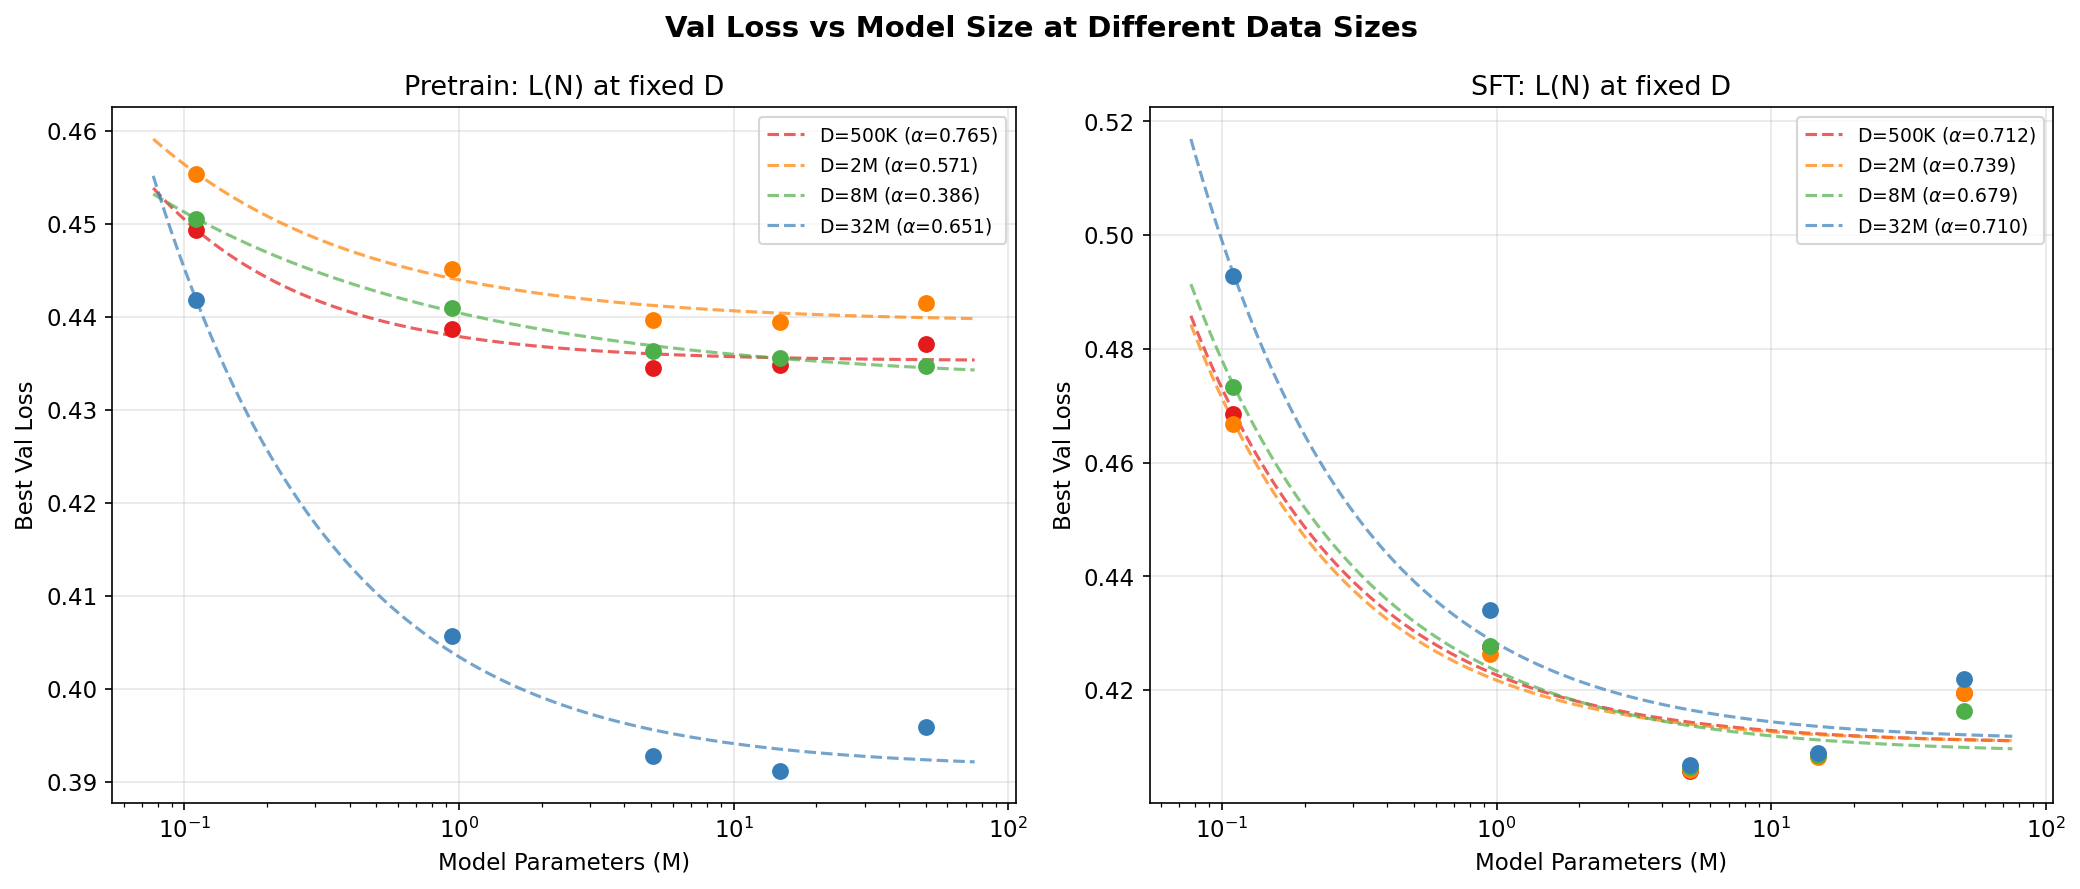
\includegraphics[width=\textwidth]{scaling_law_nd.png}
\caption{\textbf{Pretraining and SFT scaling laws.} Minimum validation NLL loss versus model
size for pretrain (left) and SFT (right) at four dataset sizes (500K, 2M, 8M, 32M). Dashed
lines show power law fits $L(N) = a \cdot N^{-\alpha} + c$. Points represent individual runs;
each configuration was run once.}
\label{fig:scaling_nd}
\end{figure}

\begin{table}[H]
\centering
\caption{Power law fit parameters for pretraining and SFT scaling laws.
Form: $L(N) = a \cdot N^{-\alpha} + c$.
Dashes indicate $c$ was not reliably estimated and was omitted ($c = 0$).}
\label{tab:fits}
\begin{tabular}{lccc|ccc}
\toprule
 & \multicolumn{3}{c|}{Pretrain} & \multicolumn{3}{c}{SFT} \\
Dataset & $a$ & $\alpha$ & $c$ & $a$ & $\alpha$ & $c$ \\
\midrule
500K & 0.0026 & 0.765 & --     & 0.0121 & 0.712 & -- \\
2M   & 0.0045 & 0.572 & 0.4394 & 0.0111 & 0.739 & -- \\
8M   & 0.0076 & 0.386 & --     & 0.0145 & 0.679 & -- \\
32M  & 0.0120 & 0.651 & --     & 0.0171 & 0.710 & -- \\
\bottomrule
\end{tabular}
\end{table}

Pretraining validation loss decreases as a power law in model size at all four dataset sizes.
The effect is most pronounced at 32M sequences: the 15M model achieves a minimum validation
loss of 0.391, compared to 0.442 for the 0.1M model, a reduction of 0.051 NLL units.
At smaller dataset sizes the improvement is more modest: at 8M sequences, all five model
sizes converge to validation losses between 0.435 and 0.451 (a span of only 0.016 NLL units),
reflecting a data-limited regime in which even the smallest model extracts most of the
available signal.

The fitted scaling exponent $\alpha$ varies across dataset sizes: 0.765 (500K), 0.572 (2M),
0.386 (8M), and 0.651 (32M). The shallow exponent at 8M reflects the near-convergence of
model sizes under that training regime. At 32M, the wider spread of validation losses (range
0.051) supports a steeper fitted exponent. The non-monotonic pattern of $\alpha$ with dataset
size suggests that the relative benefit of model scale depends on the data volume available:
when data is abundant (32M), larger models pull further ahead; when data is limited
(8M in our range), capacity differences are compressed.

A notable observation is that the 50M-parameter model performs worse than the 15M model at
all four dataset sizes under equivalent hyperparameters (0.437 vs.\ 0.435 at 500K;
0.441 vs.\ 0.439 at 2M; 0.438 vs.\ 0.436 at 8M; 0.396 vs.\ 0.391 at 32M). In the scaling
law figure, the 50M/8M point appears to beat 15M (0.435 vs.\ 0.436); however, this is
because that run used a tuned learning rate of $3\times10^{-5}$ rather than the standard
$1\times10^{-5}$, identified via a sensitivity analysis. With the standard LR, the 50M model
at 8M achieves 0.438, consistent with the pattern across other dataset sizes. This behavior is consistent with data starvation. Applying the compute-optimal
prescription of Hoffmann et al.~\cite{hoffmann2022} ($D \approx 20N$ tokens), our pretraining
budget of approximately 164M tokens is compute-optimal only for a model of approximately 8M
parameters. Every model larger than 5M parameters is under-trained relative to its capacity:
the 15M model requires $\sim$300M tokens (1.8$\times$ our budget) and the 50M model requires
$\sim$1B tokens (6$\times$ our budget). The 50M model's underperformance relative to 15M
therefore does not indicate that 15M is well-trained (both are data-starved) but that 50M
is considerably more starved. The true remedy is scaling dataset size and training steps
together with model size, consistent with the compute-optimal prescription.

\subsection{SFT Scaling Laws}

Validation loss after SFT also follows a power law in model size (Table~\ref{tab:fits},
right), with exponents in the range 0.68--0.74 across dataset sizes. Figure~\ref{fig:scaling_2m}
shows pretraining and SFT scaling curves at the 2M dataset on a shared y-axis, making the
difference in steepness directly visible: the SFT curve drops more steeply with model size
than the pretraining curve, consistent with the higher $\alpha$ values.

\begin{figure}[H]
\centering
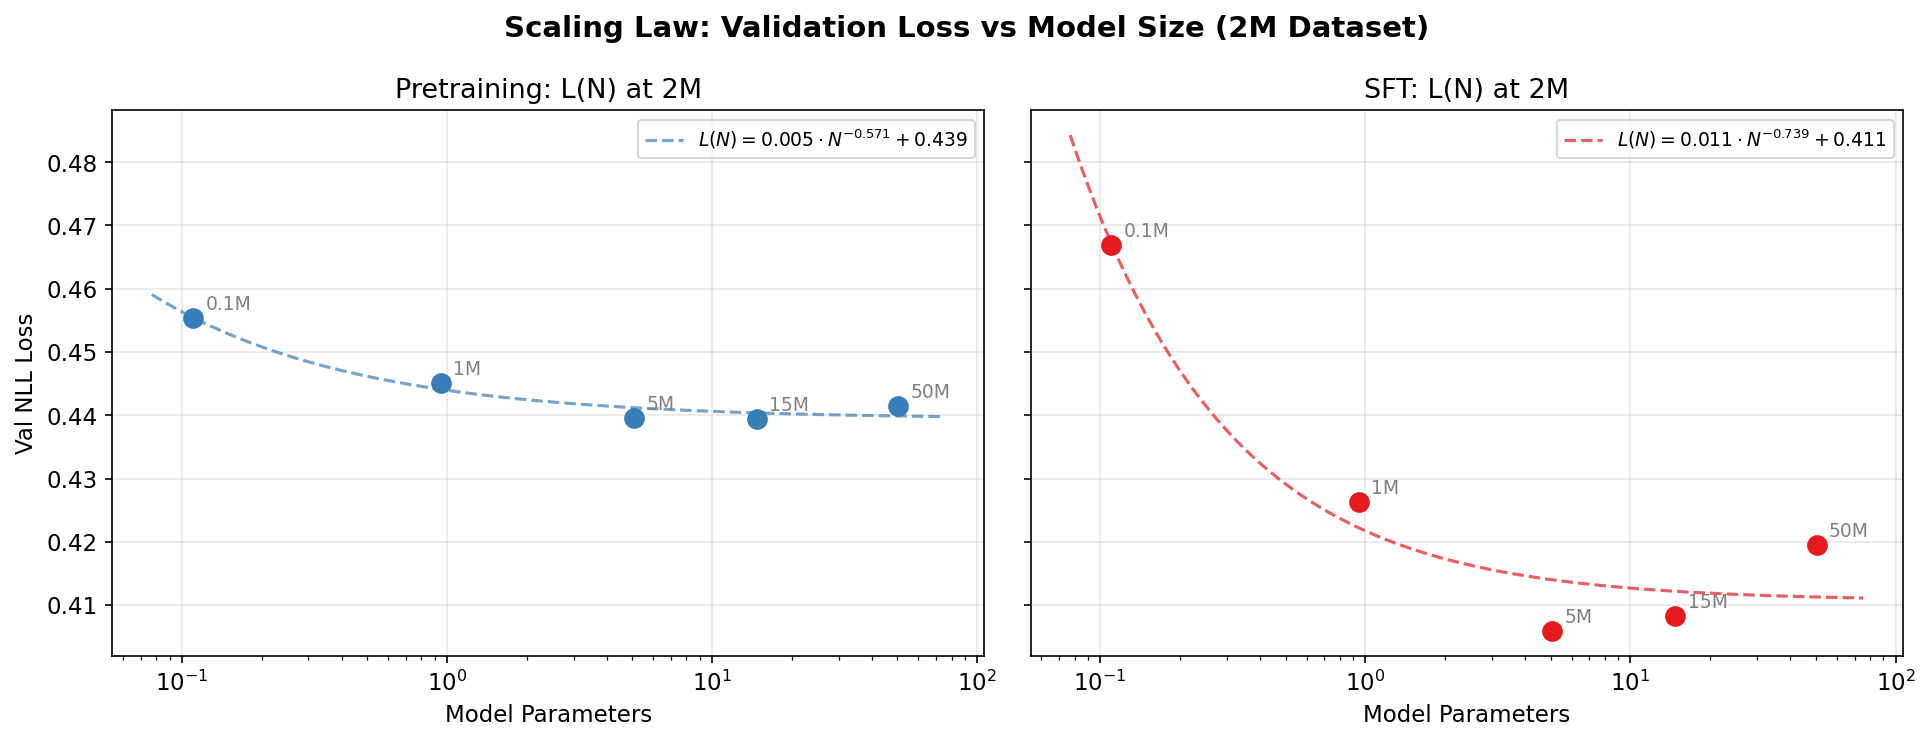
\includegraphics[width=\textwidth]{scaling_law_2m.png}
\caption{\textbf{Pretraining vs.\ SFT scaling at the 2M dataset.} Both panels share the same
y-axis scale, making the steeper descent of the SFT curve (right, $\alpha = 0.739$) relative
to the pretraining curve (left, $\alpha = 0.572$) directly visible. A steeper curve indicates
that model scale is a more effective lever for conditional generation than for unconditional
pretraining.}
\label{fig:scaling_2m}
\end{figure}

These SFT exponents
exceed the corresponding pretrain exponents at every dataset size except 500K, where both
are similar ($\alpha = 0.765$ pretrain vs.\ 0.712 SFT). This finding indicates that
conditional generation benefits from model capacity at least as much as, and in most
conditions proportionally more than, unconditional sequence modeling.

A striking non-monotonicity appears in the SFT results: the 5M-parameter model achieves the
lowest SFT validation loss across all four dataset sizes (0.406, 0.406, 0.406, and 0.407 at
500K, 2M, 8M, and 32M, respectively), outperforming both the 15M (average 0.409) and 50M
(average 0.419) models. This suggests that for the available SFT data volume, the 5M model
is closest to the compute-optimal configuration for fine-tuning. The larger models likely
underperform at SFT due to data starvation at the fine-tuning stage: the SFT training set
contains far fewer examples than the pretraining corpus, and models with greater capacity
are unable to fully utilize it.

\subsection{Generation Quality}

Figure~\ref{fig:eval_n} shows mean evaluation metrics for generated TCR sequences as a
function of model size, and Figure~\ref{fig:eval_d} shows the same metrics as a function of
dataset size.

\begin{figure}[H]
\centering
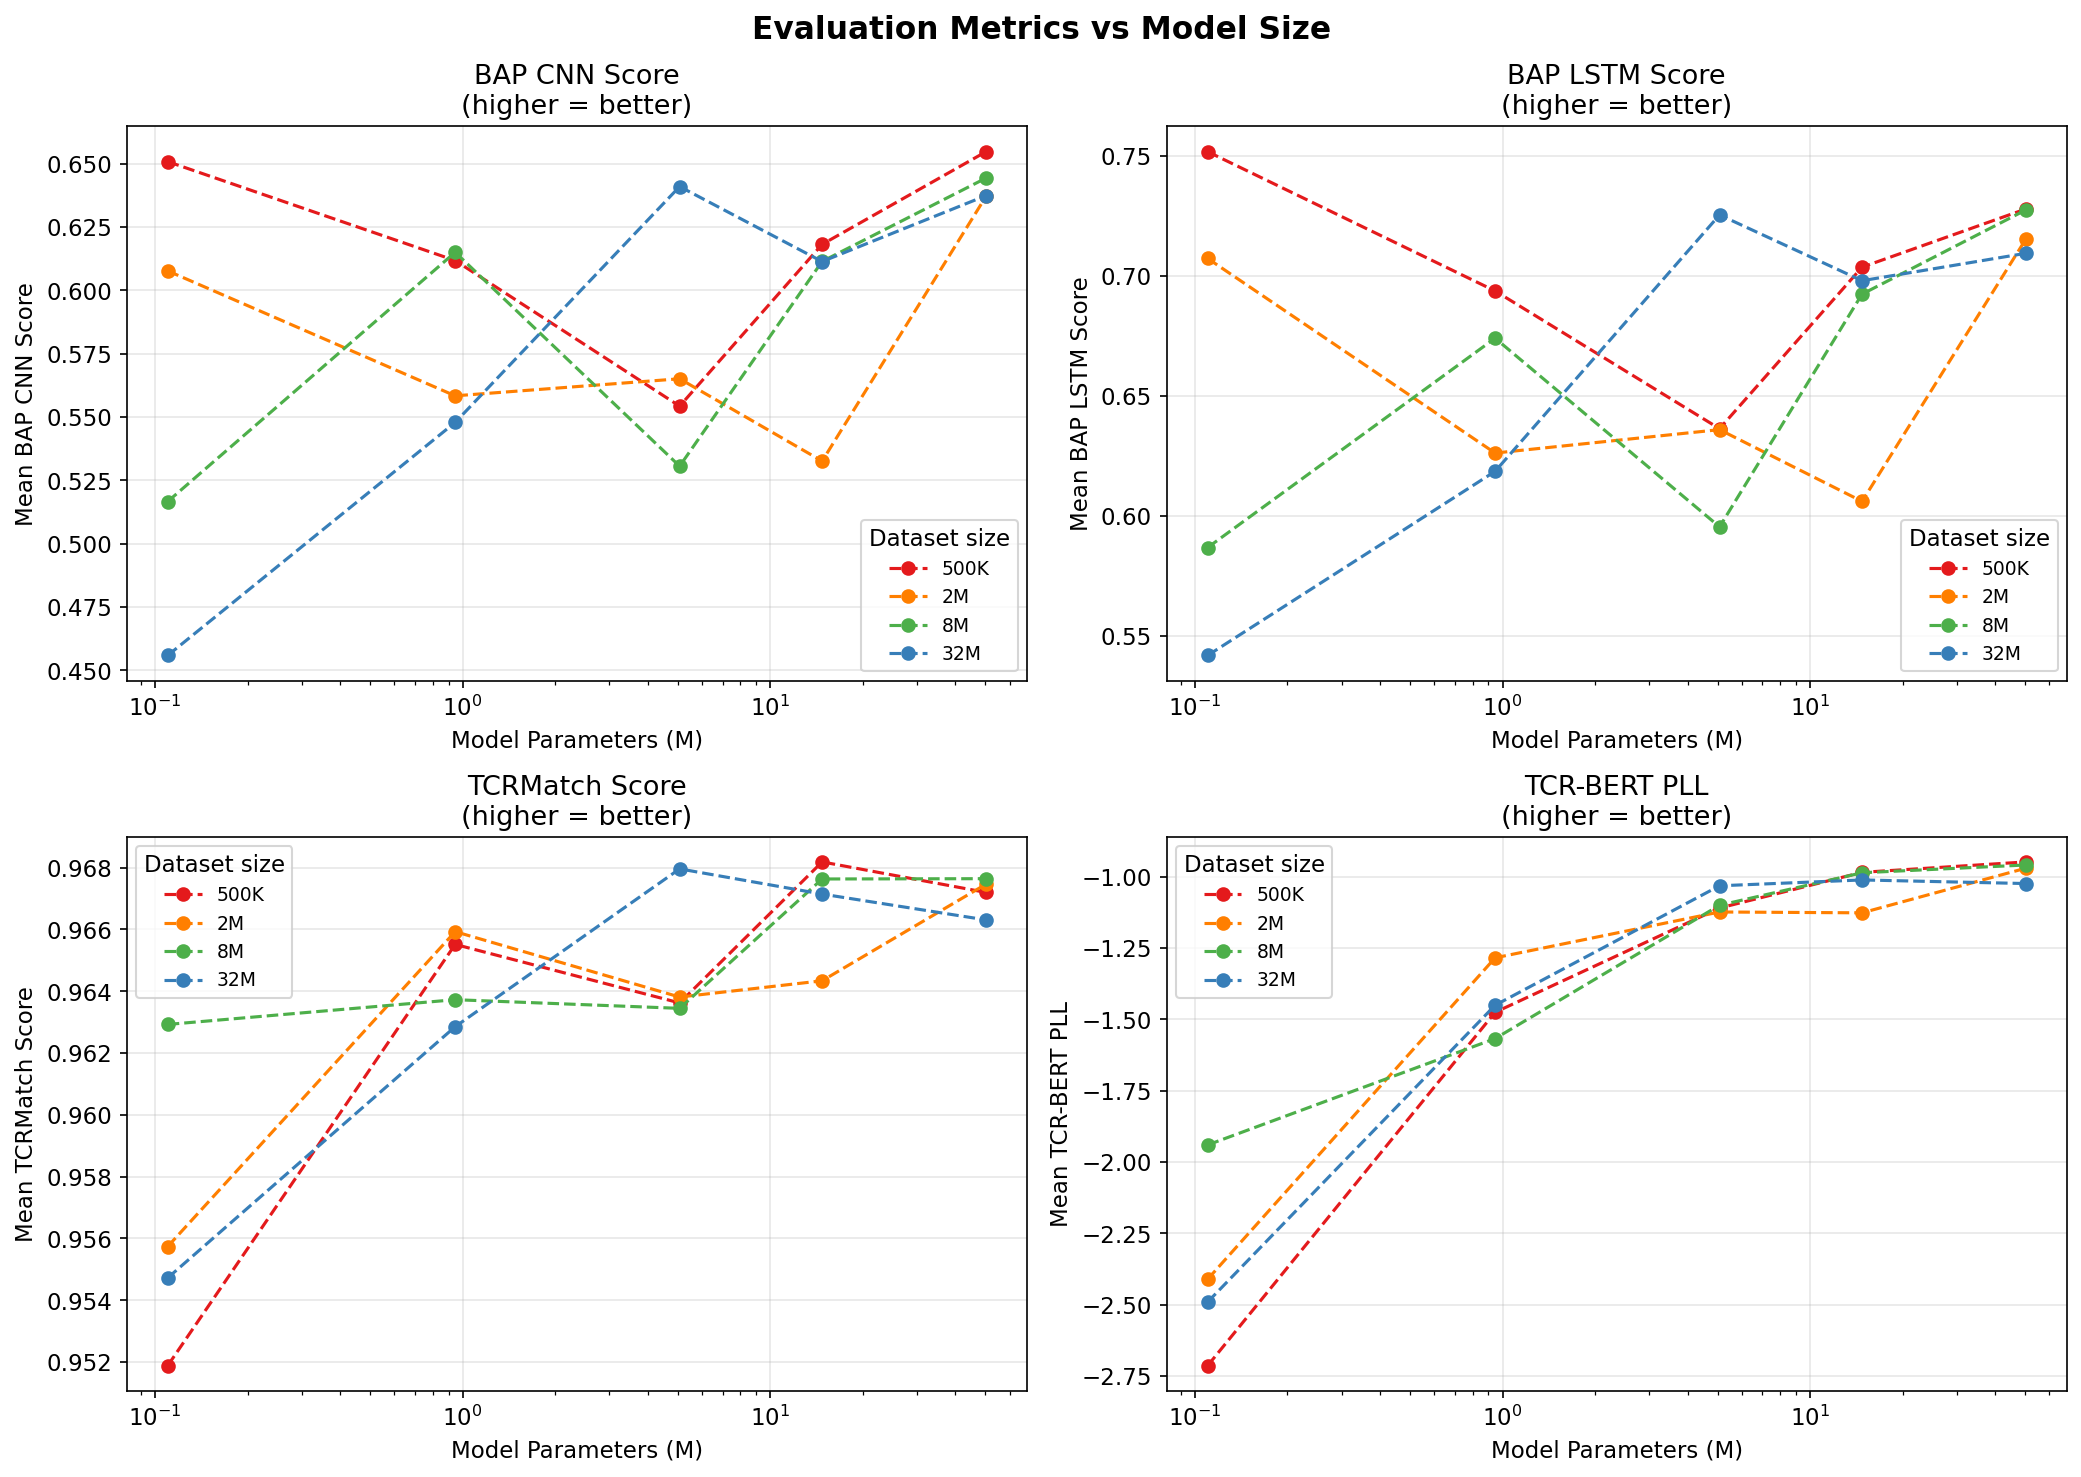
\includegraphics[width=\textwidth]{eval_vs_n.png}
\caption{\textbf{Generation quality versus model size.} Mean BAP CNN score, BAP LSTM score,
TCRMatch score, and TCR-BERT MLM pseudo-log-likelihood (primary metric) for each model size
at four dataset sizes. Each point represents the mean over 15 test epitopes $\times$ 100
generated sequences per epitope.}
\label{fig:eval_n}
\end{figure}

\begin{table}[H]
\centering
\caption{Mean evaluation metrics for generated TCR sequences across all 20 SFT model
configurations. Metrics are averaged over 15 test epitopes and $\sim$100 generated sequences
per epitope. Higher values are better for all metrics. Bold indicates the best value in each
column.}
\label{tab:eval}
\begin{tabular}{llcccc}
\toprule
Size & Dataset & BAP CNN & BAP LSTM & TCRMatch & BERT PLL \\
\midrule
0.1M & 500K & 0.651 & 0.752 & 0.952 & $-2.714$ \\
0.1M & 2M   & 0.608 & 0.707 & 0.956 & $-2.411$ \\
0.1M & 8M   & 0.517 & 0.587 & 0.963 & $-1.940$ \\
0.1M & 32M  & 0.456 & 0.542 & 0.955 & $-2.491$ \\
\midrule
1M   & 500K & 0.612 & 0.694 & 0.966 & $-1.476$ \\
1M   & 2M   & 0.558 & 0.626 & 0.966 & $-1.285$ \\
1M   & 8M   & 0.615 & 0.674 & 0.964 & $-1.568$ \\
1M   & 32M  & 0.548 & 0.619 & 0.963 & $-1.451$ \\
\midrule
5M   & 500K & 0.554 & 0.636 & 0.964 & $-1.110$ \\
5M   & 2M   & 0.565 & 0.636 & 0.964 & $-1.124$ \\
5M   & 8M   & 0.531 & 0.596 & 0.963 & $-1.100$ \\
5M   & 32M  & 0.641 & 0.726 & 0.968 & $-1.032$ \\
\midrule
15M  & 500K & 0.618 & 0.704 & \textbf{0.968} & $-0.985$ \\
15M  & 2M   & 0.533 & 0.606 & 0.964 & $-1.127$ \\
15M  & 8M   & 0.611 & 0.693 & \textbf{0.968} & $-0.986$ \\
15M  & 32M  & 0.611 & 0.698 & 0.967 & $-1.012$ \\
\midrule
50M  & 500K & \textbf{0.655} & \textbf{0.728} & 0.967 & $\mathbf{-0.948}$ \\
50M  & 2M   & 0.637 & 0.716 & \textbf{0.968} & $-0.970$ \\
50M  & 8M   & 0.644 & \textbf{0.728} & \textbf{0.968} & $-0.959$ \\
50M  & 32M  & 0.637 & 0.710 & 0.966 & $-1.024$ \\
\bottomrule
\end{tabular}
\end{table}

\begin{figure}[H]
\centering
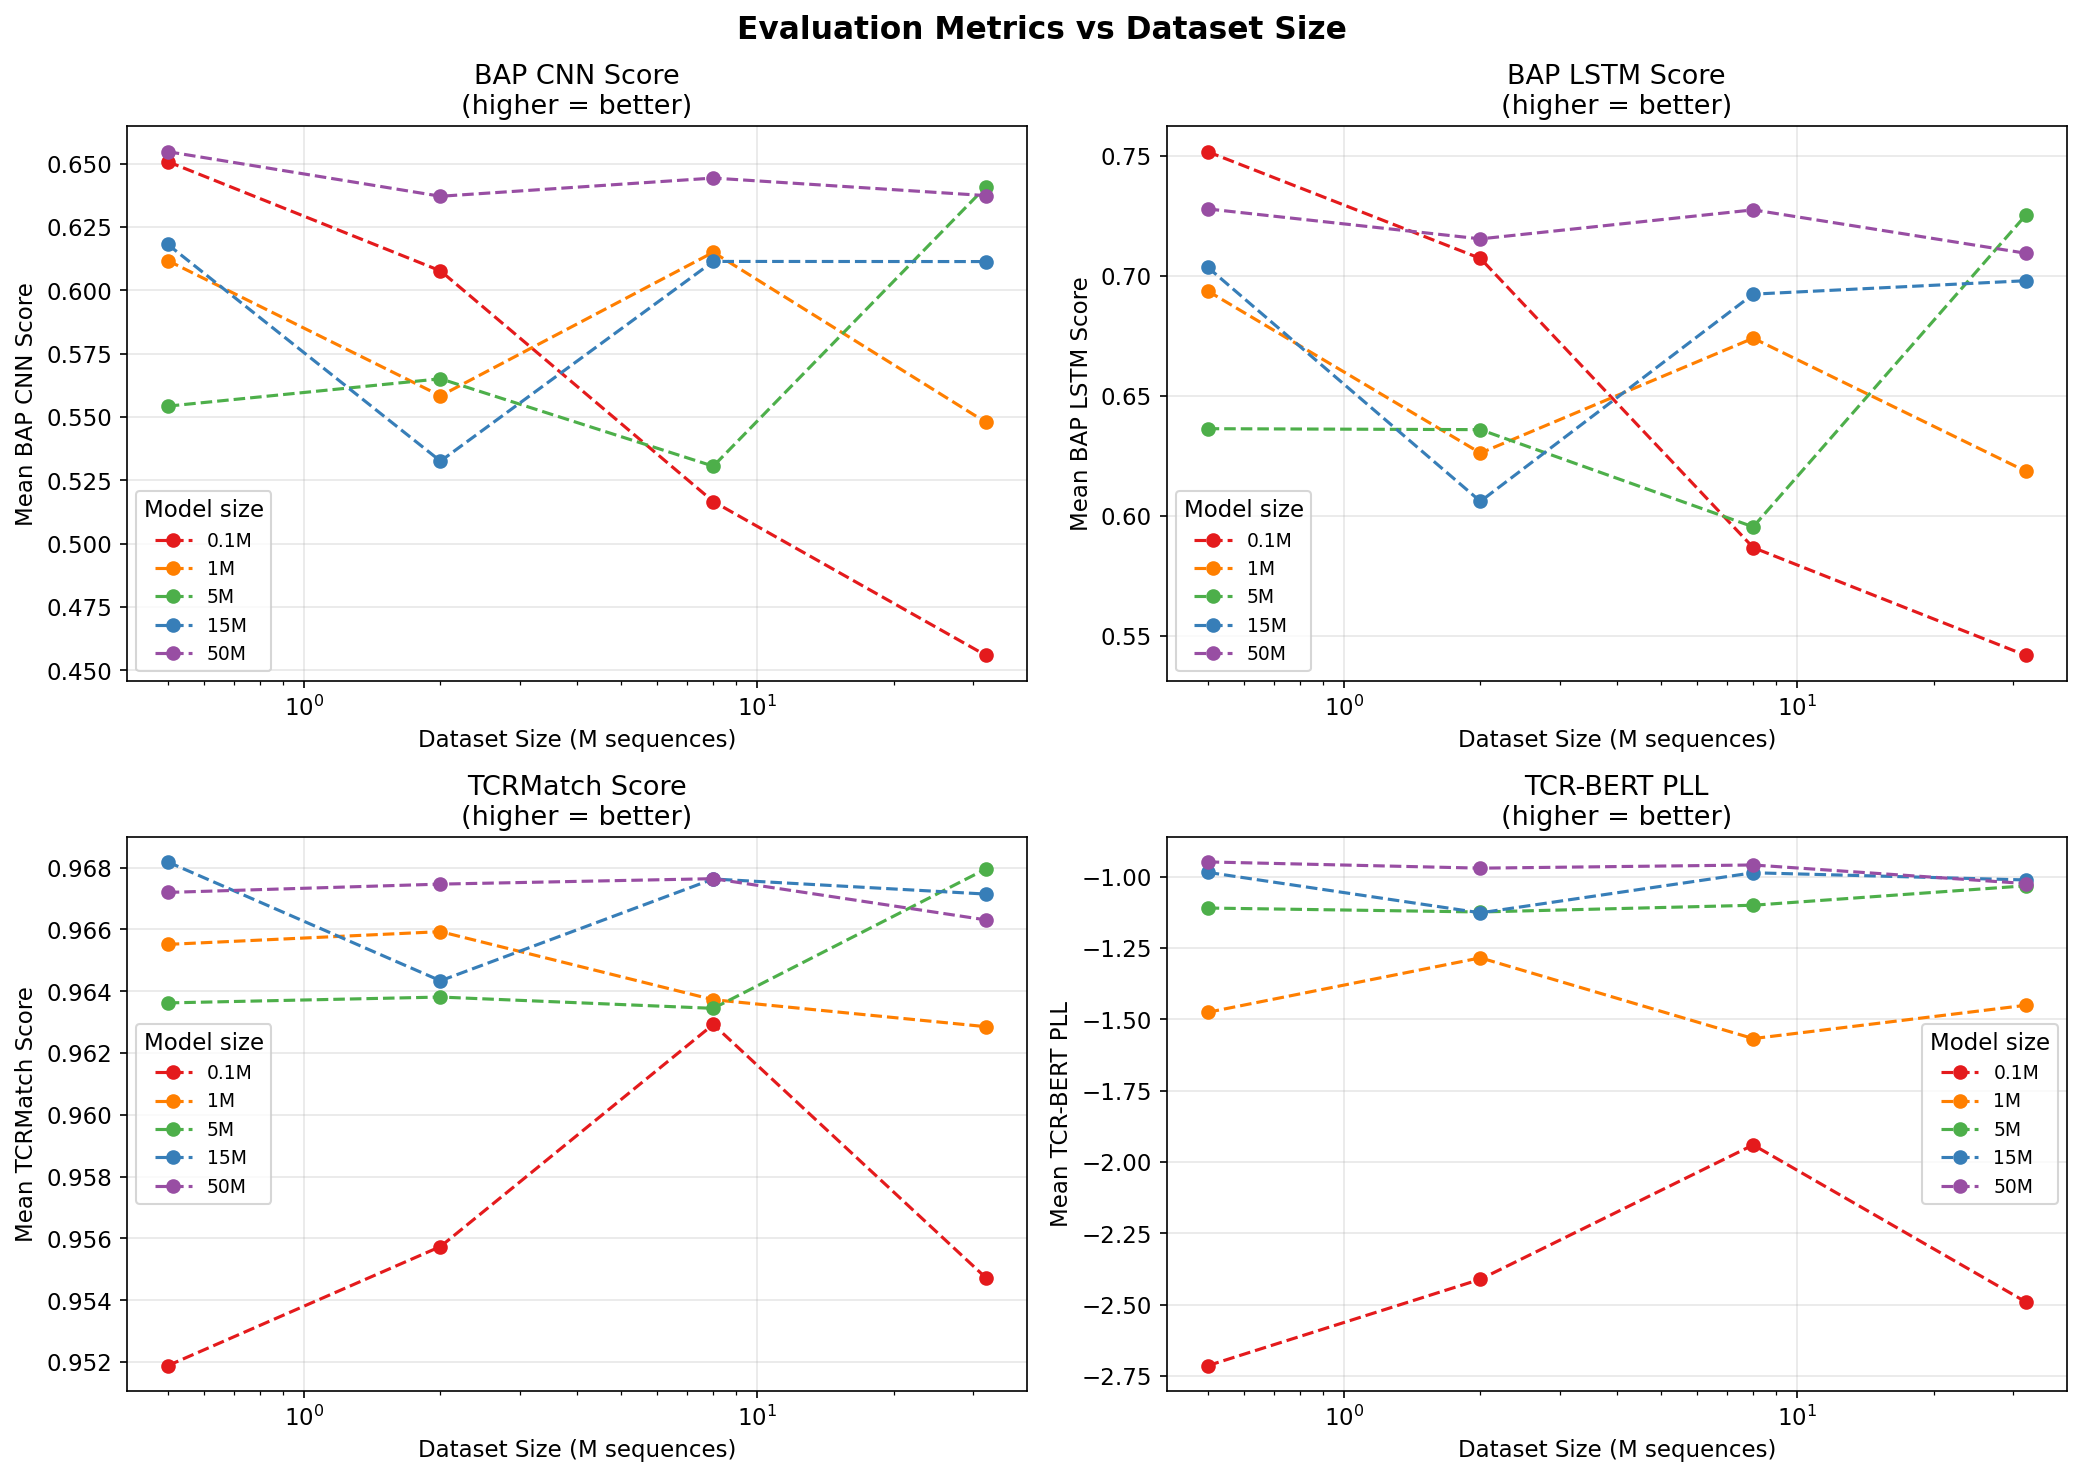
\includegraphics[width=\textwidth]{eval_vs_d.png}
\caption{\textbf{Generation quality versus dataset size.} Same metrics as
Figure~\ref{fig:eval_n}, plotted as a function of dataset size for each model size.}
\label{fig:eval_d}
\end{figure}

\textbf{TCR-BERT pseudo-log-likelihood} (primary metric) improves monotonically with model
size across all dataset sizes. The 50M model achieves a mean PLL of $-0.975$ nats (averaged
across the four dataset sizes), compared to $-2.389$ nats for the 0.1M model, a gain of
1.41 nats. The 15M and 50M models achieve similar PLL scores ($-1.028$ and $-0.975$ nats,
respectively), consistent with diminishing returns at large model size. The best individual
result (50M model trained on the 500K dataset) achieves a mean PLL of $-0.948$ nats.

\textbf{Binding Affinity Prediction.} BAP CNN scores range from 0.46 (0.1M/32M) to 0.65
(50M/500K), and BAP LSTM scores range from 0.54 to 0.73 across all model--dataset
combinations. The 50M model consistently achieves the highest BAP scores. BAP CNN and LSTM
scores are broadly concordant with TCR-BERT PLL ordering across model sizes, though they
are noisier, particularly for the 0.1M model, where high BAP scores may reflect a different
failure mode (generating high-affinity but low-diversity sequences).

\textbf{TCRMatch.} BLOSUM62 similarity to known TCR binders is uniformly high across all
models and dataset sizes (range: 0.952--0.968), with no clear trend with model size or
dataset size. The narrow range of TCRMatch scores indicates that all models successfully
generate CDR3$\beta$-like sequences; the metric is not a sensitive discriminator of
generation quality in our setting.

\textbf{Dataset size effects on generation quality.} Generation quality shows a weaker and
less consistent dependence on pretraining dataset size than on model size
(Figure~\ref{fig:eval_d}). For the 50M model, TCR-BERT PLL varies by only 0.076 nats across
the four dataset sizes ($-0.948$ at 500K, $-0.970$ at 2M, $-0.959$ at 8M, $-1.024$ at
32M). The absence of a consistent monotonic trend with dataset size suggests that, in the
range studied, generation quality is more sensitive to model capacity than to the volume of
pretraining data.

% ===========================================================================
% DISCUSSION
% ===========================================================================
\section{Discussion}

\textbf{Scaling law exponents relative to NLP.}
The pretraining exponents we observe ($\alpha = 0.39$--$0.77$) are substantially larger
than those reported by Kaplan et al.~\cite{kaplan2020} for autoregressive language models
($\alpha \approx 0.076$) trained on English text. Two factors likely explain this difference.
First, TCR CDR3 sequences are short (mean 15 amino acids) and structurally constrained by
the conserved CASS prefix and J-gene-encoded suffix; the effective information content per
token is lower than in natural language. Modest-sized models can therefore quickly saturate
the available signal at small dataset sizes, compressing the range of validation losses and
inflating the fitted exponent. Second, our model size range (0.1M--50M parameters) is
orders of magnitude smaller than the scales studied by Kaplan et al. (up to 1.5B parameters),
and power law exponents can vary substantially with the range of scales examined.

The SFT exponents ($\alpha = 0.68$--$0.74$) exceed pretrain exponents in most conditions,
indicating that epitope-conditioned TCR generation benefits proportionally more from model
capacity than does unconditional sequence modeling. A natural interpretation is that
conditional generation is a harder task: the model must learn not only the marginal
distribution of TCR sequences but the joint distribution conditioned on epitope identity,
requiring greater representational capacity for the same level of generalization.

\textbf{Data starvation and compute-optimal scaling.}
The underperformance of the 50M model relative to the 15M model is consistent with the
compute-optimal scaling analysis of Hoffmann et al.~\cite{hoffmann2022}, who showed that
efficient utilization of a model with $N$ parameters requires approximately $20N$ training
tokens. Our budget of 164M tokens is compute-optimal for a model of approximately 8M
parameters. Both the 15M model ($\sim$300M tokens needed, 1.8$\times$ our budget) and the
50M model ($\sim$1B tokens needed, 6$\times$ our budget) are under-trained relative to their
capacity. The 50M model underperforms 15M not because 15M is well-trained, but because 15M is
considerably less starved.
The same reasoning applies to SFT: the SFT corpus contains tens of thousands of
epitope-TCR pairs, far fewer than the number that would compute-optimally train a 50M-parameter
model.

The current experimental design — holding training budget fixed while scaling model size —
is structurally unable to isolate capacity effects: small models are inevitably over-trained
and large models are inevitably under-trained, regardless of hyperparameter tuning. Future
work will move to an isoFLOP experimental design~\cite{hoffmann2022}: fix a total compute
budget (FLOPs), then for each budget level identify the optimal (model size, training tokens)
pair. By construction, every point on the resulting scaling curve is compute-optimal, making
comparisons across model sizes meaningful rather than confounded by differential training
adequacy. This is the experimental paradigm used by Hoffmann et al.~\cite{hoffmann2022} and
represents the appropriate framework for characterizing true capacity scaling in DPLM models.

\textbf{Hyperparameter sensitivity and learning rate tuning.}
Learning rates in this study were set by hand based on the heuristic of scaling LR down with
model size, without systematic validation. The one configuration where two learning rates were
compared (the 50M model on the 8M dataset) revealed that a $3\times$ difference in LR
changed the validation loss enough to alter which model size won that comparison (with the
standard LR of $1\times10^{-5}$, the 50M model achieves val loss 0.438, worse than the 15M
model at 0.436; with the tuned LR of $3\times10^{-5}$, 50M achieves 0.435, edging out 15M).
This finding suggests that the other 19 pretrain configurations may also not be at their
optimal learning rates, which means the fitted scaling law exponents should be interpreted
with this caveat in mind: they reflect model capacity under a single hyperparameter guess
per configuration, not under optimal hyperparameters. Future work will address this by
performing a systematic learning rate sweep for each model size before running the full
scaling grid, ensuring that each data point reflects the model's true capacity and yielding
more reliable scaling law exponents.

\textbf{Limitations of cross-dataset validation loss comparisons.}
Each dataset size uses a different validation set (a 20\% random split of its own training
pool). This design precludes direct comparison of validation losses across dataset sizes: the
validation set at 500K contains 100K sequences from a different distribution than the
validation set at 32M, which contains 6.4M sequences from a different source file entirely.
Unlike Kaplan et al.~\cite{kaplan2020} and Hoffmann et al.~\cite{hoffmann2022}, who hold the
evaluation set constant when fitting $L(D)$ curves, our experimental setup confounds
dataset size with validation set composition. Consequently, we do not report $L(D)$ power
law fits. Our $L(N)$ fits at a given dataset size are internally valid because all five
model sizes share the same validation set, but $L(D)$ comparisons across dataset sizes would
not be interpretable.

\textbf{Evaluation metric sensitivity.}
The near-uniform TCRMatch scores (0.952--0.968) across all model and dataset configurations
indicate that all trained models successfully learn the CDR3$\beta$ sequence grammar: the
CASS prefix, variable CDR3 core, and conserved J-gene suffix. TCRMatch thus serves primarily
as a quality filter (confirming that generation is not degenerate) rather than a sensitive
measure of improvement. TCR-BERT PLL provides more discriminative signal and is arguably the
most biologically relevant measure of the generated sequences' plausibility as natural TCRs,
independent of the generating model. BAP scores provide functional information about predicted
binding but are noisier, as the underlying BAP models were trained on a different set of
TCR-epitope pairs and may not generalize uniformly to all generated sequences.

% ===========================================================================
% CONCLUSION
% ===========================================================================
\section{Conclusion}

This thesis characterized the scaling behavior of Diffusion Protein Language Models trained
on T-cell receptor CDR3 beta chain sequences and developed a supervised fine-tuning approach
for epitope-conditioned TCR generation. Key findings are as follows.

Pretraining validation loss follows a power law in model size with exponents
$\alpha = 0.39$--$0.77$ depending on dataset size, substantially larger than typical
natural language exponents, consistent with the shorter, more constrained structure of TCR
sequences and the relatively small model sizes studied. SFT scaling exponents ($\alpha =
0.68$--$0.74$) consistently exceed pretraining exponents, indicating that conditional
generation benefits proportionally more from model capacity than does unconditional sequence
modeling. The 50M-parameter model underperforms the 15M model across all dataset sizes under
equivalent hyperparameters, consistent with compute-optimal scaling theory and the
insufficient training budget relative to model size. Conditional generation quality measured by
TCR-BERT pseudo-log-likelihood improves monotonically with model size, with the 50M model
achieving the highest sequence plausibility scores.

These results suggest that scaling model capacity is an effective strategy for improving
DPLM-based TCR generation quality, and that supervised fine-tuning for conditional generation
can be achieved with moderate epitope-TCR datasets. Future work should adopt an isoFLOP experimental design: rather than holding training budget
fixed while varying model size, fix a total compute budget and identify the optimal
(model size, training tokens) pair at each budget level. This ensures every point on the
scaling curve is compute-optimal by construction, yielding scaling law exponents that reflect
genuine capacity differences rather than differential training adequacy. Additional directions
include systematic learning rate sweeps to ensure each configuration is at its optimal
hyperparameters, expanded SFT datasets to reduce data starvation at fine-tuning, and
structure-based validation using TCR-pMHC complex structure prediction to assess the physical
binding plausibility of generated sequences.

% ===========================================================================
% REFERENCES
% ===========================================================================
\newpage
\bibliographystyle{unsrtnat}
\bibliography{references}

\end{document}
